\documentclass[a4paper]{scrartcl}
\usepackage[cm]{fullpage}
\usepackage{amsmath, amssymb, esint}
\usepackage{siunitx}

\usepackage{tikz, pgfplots}
\pgfplotsset{compat = 1.12}

\begin{document}

\title{PHYS3112: Compton Effect}
\author{ \\ \\ }
\date{2017-05-08}
\maketitle

\begin{abstract}
    Radiation from a \SI{662}{\kilo\electronvolt} gamma ray source was directed at various angles at a steel rod to validate the Compton effect. Our results agree with the Compton shift formula to a certain extent.
\end{abstract}

\section{Materials and Methods}
Please refer to the operating instructions of the experiment.

The raw data measured was smoothed with a 51-point window cubic Savitzky--Golay filter, before peaks and FWHM measurements were extracted, and then converted to \si{\kilo\electronvolt} values. All error values quoted will be these FWHM values.

Data was collected for around 20 to 30 minutes per measurement.

The peaks around \SI{75}{\kilo\electronvolt} have been ignored, since this is a characteristic line of the scintillator itself.

\section{Results}
\begin{figure}
    \centering
    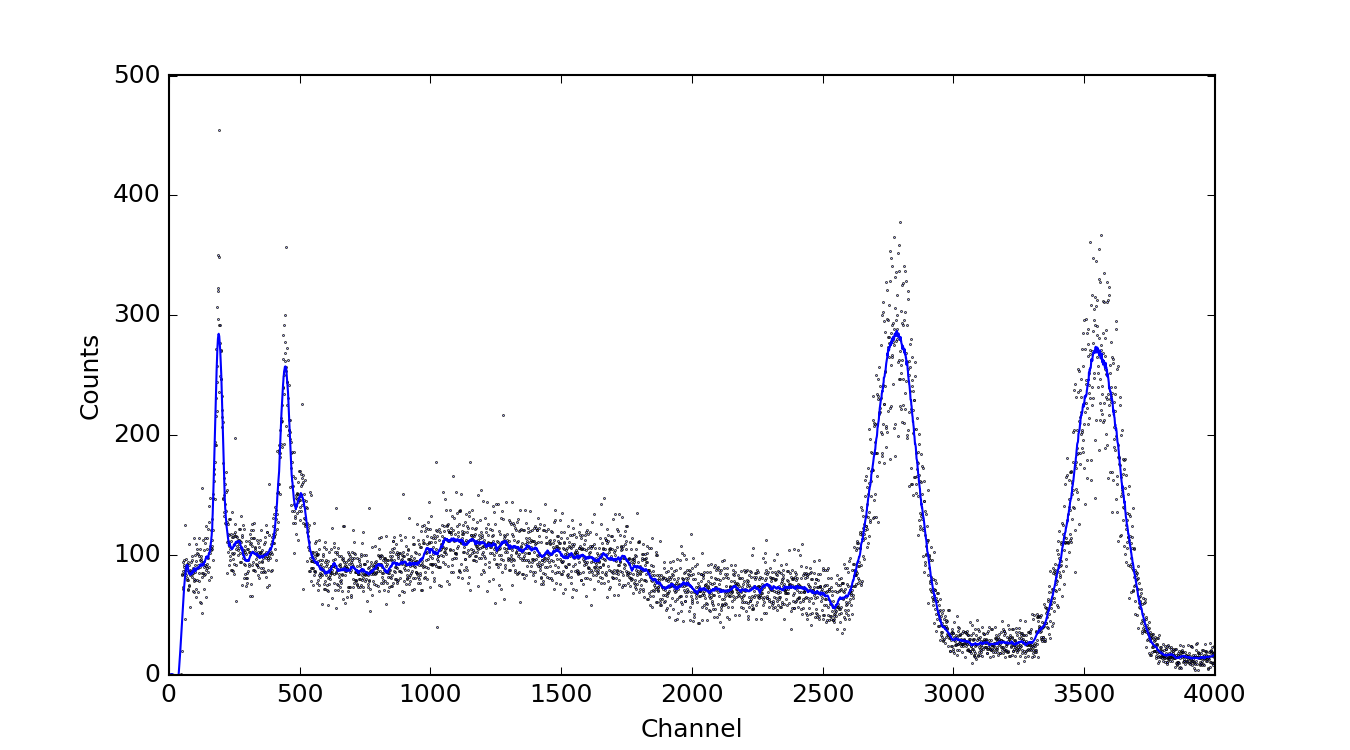
\includegraphics[height = 10cm]{data/calibration.png}
    \caption{Calibration data}
    \label{fig:calibration}
\end{figure}

\begin{figure}
    \centering
    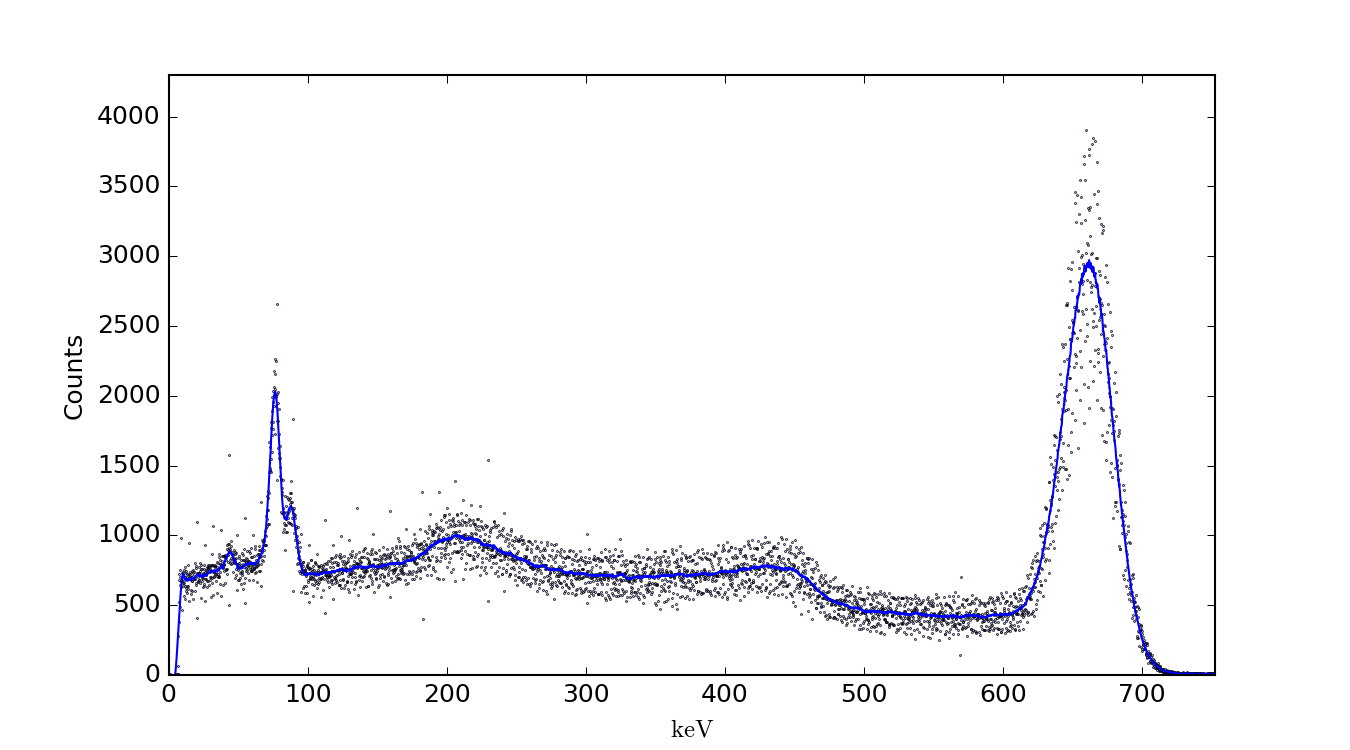
\includegraphics[height = 10cm]{data/0-no-rod.png}
    \caption{Control measurement without the steel rod}
    \label{fig:control}
\end{figure}

\begin{figure}
    \centering
    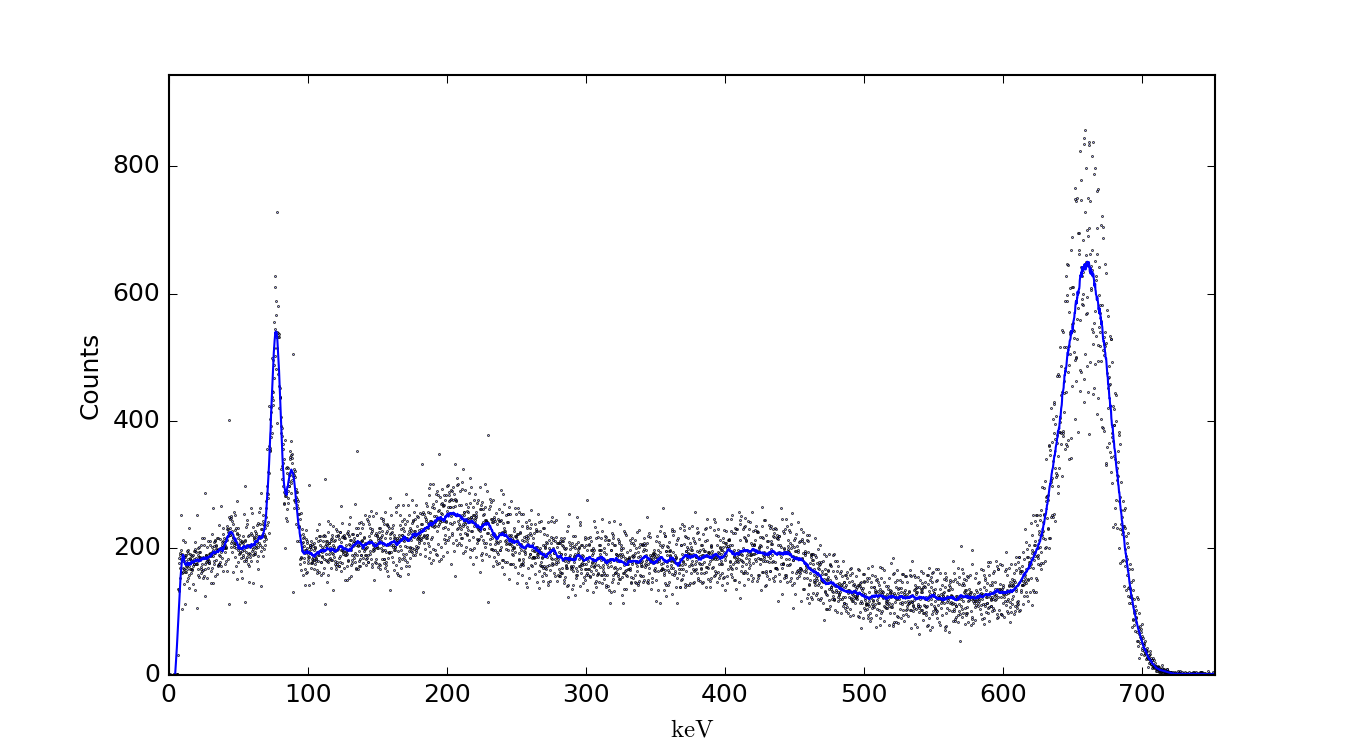
\includegraphics[height = 10cm]{data/0.png}
    \caption{\(\theta = \SI{0}{\degree}\)}
    \label{fig:0}
\end{figure}
\begin{figure}
    \centering
    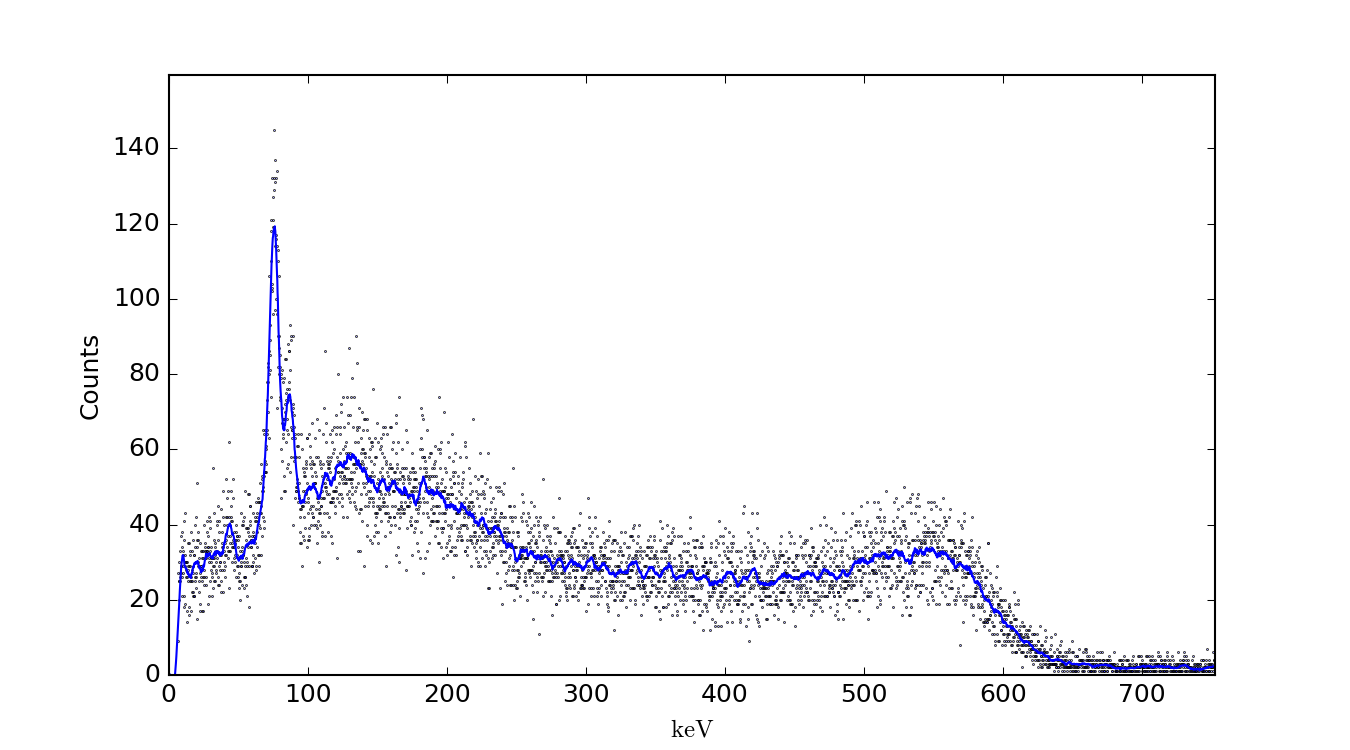
\includegraphics[height = 10cm]{data/30.png}
    \caption{\(\theta = \SI{30}{\degree}\)}
    \label{fig:30}
\end{figure}
\begin{figure}
    \centering
    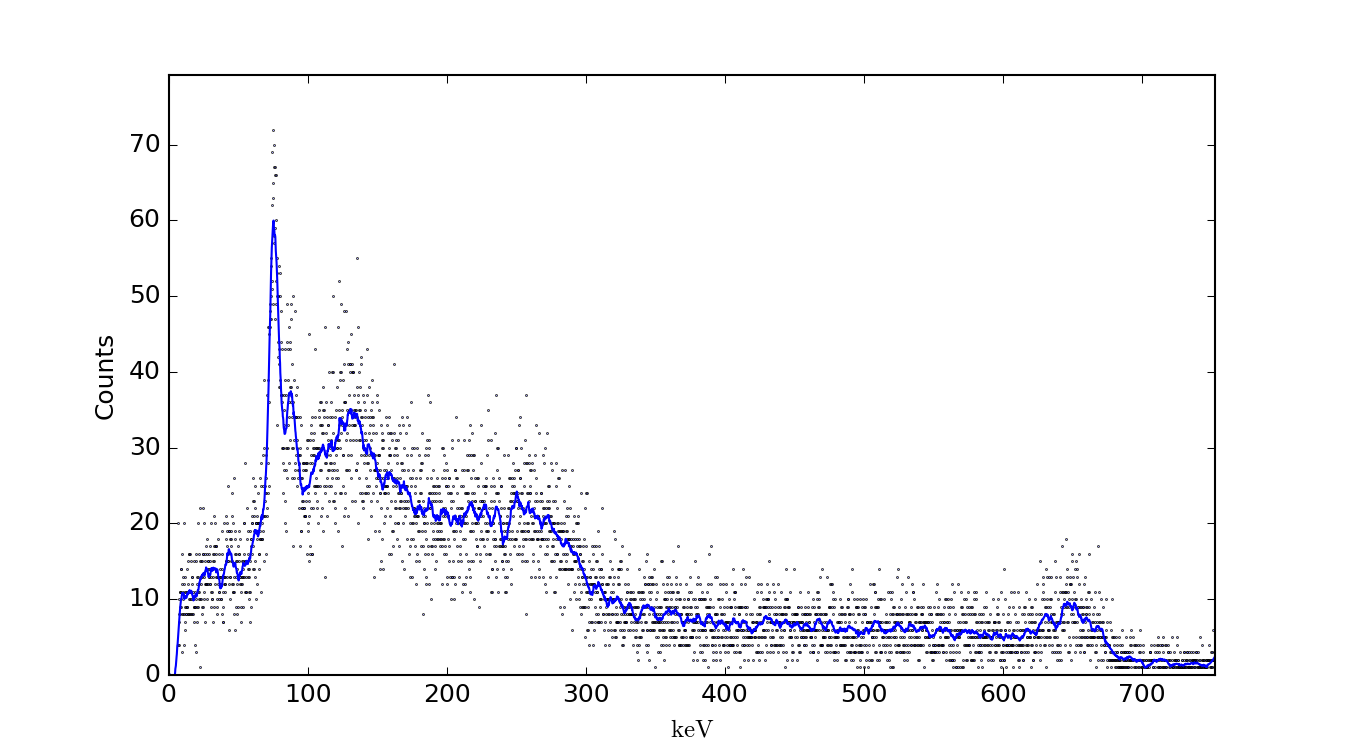
\includegraphics[height = 10cm]{data/90.png}
    \caption{\(\theta = \SI{90}{\degree}\)}
    \label{fig:90}
\end{figure}
\begin{figure}
    \centering
    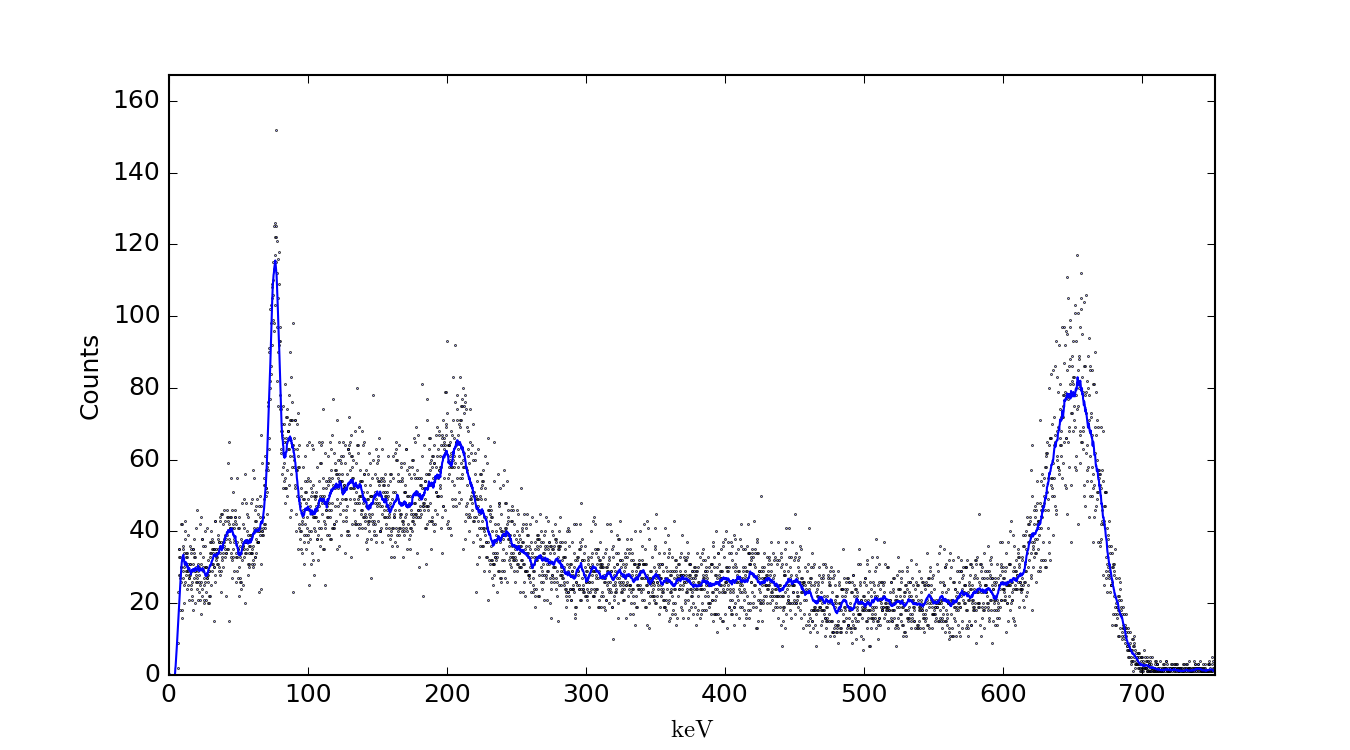
\includegraphics[height = 10cm]{data/130.png}
    \caption{\(\theta = \SI{130}{\degree}\)}
    \label{fig:130}
\end{figure}

From the calibration results in Figure \ref{fig:calibration}, the three peaks of interest are at channels \SI{192 \pm 47}{}, \SI{2771 \pm 210}{} and \SI{3545 \pm 217}{}, corresponding to the frequencies 32, 511 and \SI{662}{\kilo\electronvolt} respectively. For simplicity, if we ignore the errors in the peaks, this results in a channel-to-keV function of:
\[(-2.17522 + 0.17746 \:c + 2.79139 \times 10^-6 \:c^2) \:\si{\kilo\electronvolt}\]

A control measurement was taken at \(\theta = \SI{0}{\degree}\) both with and without the steel rod, which can be seen in Figures \ref{fig:0} and \ref{fig:control}. The figures are quite similar to each other, both containing a clear peak at \SI{660 \pm 45}{\kilo\electronvolt}.

For \(\theta = \SI{30}{\degree}\), one can observe a very minor peak at around \SI{548}{\kilo\electronvolt}, but is so minor that its FWHM is \SI{587}{\kilo\electronvolt} - larger than the value itself.

For \(\theta = \SI{90}{\degree}\), one can observe a peak at \SI{647 \pm 61}{\kilo\electronvolt}, as well as a very minor peak at around \SI{250}{\kilo\electronvolt}. This minor peak is, like the \(\theta = \SI{30}{\degree}\) peak, so minor that its FWHM is \SI{263}{\kilo\electronvolt} - larger than the value itself.

Finally for \(\theta = \SI{130}{\degree}\), once again we have a peak at \SI{655 \pm 48}{\kilo\electronvolt}, and a minor peak at \SI{210}{\kilo\electronvolt}. While this minor peak is significantly more defined than the previous minor peaks, its FWHM is still massive at \SI{229}{\kilo\electronvolt}.

\section{Discussion}
\begin{table}
    \centering
    \begin{tabular}{c | c | c}
        \(\theta\) (\si{\degree}) & Expected (\si{\kilo\electronvolt}) & Actual (\si{\kilo\electronvolt}) \\
        \hline
        0 & 662 & \SI{660 \pm 45}{} \\
        30 & 564 & \SI{548 \pm 587}{} \\
        90 & 288 & \SI{250 \pm 263}{} \\
        130 & 212 & \SI{210 \pm 229}{}
    \end{tabular}
    \caption{Expected and actual peaks for \SI{662}{\kilo\electronvolt}}
    \label{tab:expected-vs-actual}
\end{table}

Our control measurements match each other, and we get the expected \SI{662}{\kilo\electronvolt} peak, so the initial experimental setup was sound.

For \(\theta = \SI{30}{\degree}\), the peak at \SI{662}{\kilo\electronvolt} disappeared completely, but progressively reappeared as angle was increased. This is likely due to the radiation source getting closer and closer to the detector, and the rays directly travelling towards it (as opposed to being reflected from the steel rod). This was partially blocked by a lead block, but was difficult to do well for the larger angles.

Our primary interest, however, are in the smaller peaks, which likely correspond to the Compton shifts. From our theoretical calculations for the Compton shift with an incident beam of \SI{662}{\kilo\electronvolt}, we obtain the expected energies compared to the actual peaks shown in Table \ref{tab:expected-vs-actual}. Ignoring the FWHM values for now, they match reasonably well, indicating a valid formula.

Unfortunately, for our non-control measurements, the FWHM values for the peaks were of the same order of magnitude as the values themselves. The reason for this is that our measurements contained a significant amount of ``background'' radiation (which might have also originated from the source), and FWHM is a poor metric when background is not subtracted out.

A solution to this would be to estimate the background from the control measurements and transforming it through the Compton shift formula, and subtracting it out. An issue with this approach is that the formula does not give any indication for the energy dependence of the reflected intensity, which would require deeper theoretical analysis to determine.

One could also take measurements for a longer period of time to reduce the noise in the results so less smoothing would be required, since smoothing reduces the prominence of peaks.

\section{Conclusion}
\emph{(From abstract)} Radiation from a \SI{662}{\kilo\electronvolt} gamma ray source was directed at various angles at a steel rod to validate the Compton effect. Our results agree with the Compton shift formula to a certain extent, as can be seen in Table \ref{tab:expected-vs-actual}.

\end{document}